%File: formatting-instructions-latex-2026.tex
%release 2026.0
\documentclass[letterpaper]{article} % DO NOT CHANGE THIS
\usepackage{aaai2026}  % DO NOT CHANGE THIS
\usepackage{times}  % DO NOT CHANGE THIS
\usepackage{helvet}  % DO NOT CHANGE THIS
\usepackage{courier}  % DO NOT CHANGE THIS
\usepackage[hyphens]{url}  % DO NOT CHANGE THIS
\usepackage{graphicx} % DO NOT CHANGE THIS
\urlstyle{rm} % DO NOT CHANGE THIS
\def\UrlFont{\rm}  % DO NOT CHANGE THIS
\usepackage{natbib}  % DO NOT CHANGE THIS AND DO NOT ADD ANY OPTIONS TO IT
\usepackage{caption} % DO NOT CHANGE THIS AND DO NOT ADD ANY OPTIONS TO IT
\frenchspacing  % DO NOT CHANGE THIS
\setlength{\pdfpagewidth}{8.5in}  % DO NOT CHANGE THIS
\setlength{\pdfpageheight}{11in}  % DO NOT CHANGE THIS
%
% These are recommended to typeset algorithms but not required. See the subsubsection on algorithms. Remove them if you don't have algorithms in your paper.
\usepackage{algorithm}
\usepackage{algpseudocode}

\usepackage{booktabs}
\usepackage{adjustbox}

%
% These are are recommended to typeset listings but not required. See the subsubsection on listing. Remove this block if you don't have listings in your paper.
\usepackage{newfloat}
\usepackage{listings}
\DeclareCaptionStyle{ruled}{labelfont=normalfont,labelsep=colon,strut=off} % DO NOT CHANGE THIS
\lstset{%
	basicstyle={\footnotesize\ttfamily},% footnotesize acceptable for monospace
	numbers=left,numberstyle=\footnotesize,xleftmargin=2em,% show line numbers, remove this entire line if you don't want the numbers.
	aboveskip=0pt,belowskip=0pt,%
	showstringspaces=false,tabsize=2,breaklines=true}
\floatstyle{ruled}
\newfloat{listing}{tb}{lst}{}
\floatname{listing}{Listing}
%
% Keep the \pdfinfo as shown here. There's no need
% for you to add the /Title and /Author tags.
\pdfinfo{
/TemplateVersion (2026.1)
}

% DISALLOWED PACKAGES
% \usepackage{authblk} -- This package is specifically forbidden
% \usepackage{balance} -- This package is specifically forbidden
% \usepackage{color (if used in text)
% \usepackage{CJK} -- This package is specifically forbidden
% \usepackage{float} -- This package is specifically forbidden
% \usepackage{flushend} -- This package is specifically forbidden
% \usepackage{fontenc} -- This package is specifically forbidden
% \usepackage{fullpage} -- This package is specifically forbidden
% \usepackage{geometry} -- This package is specifically forbidden
% \usepackage{grffile} -- This package is specifically forbidden
% \usepackage{hyperref} -- This package is specifically forbidden
% \usepackage{navigator} -- This package is specifically forbidden
% (or any other package that embeds links such as navigator or hyperref)
% \indentfirst} -- This package is specifically forbidden
% \layout} -- This package is specifically forbidden
% \multicol} -- This package is specifically forbidden
% \nameref} -- This package is specifically forbidden
% \usepackage{savetrees} -- This package is specifically forbidden
% \usepackage{setspace} -- This package is specifically forbidden
% \usepackage{stfloats} -- This package is specifically forbidden
% \usepackage{tabu} -- This package is specifically forbidden
% \usepackage{titlesec} -- This package is specifically forbidden
% \usepackage{tocbibind} -- This package is specifically forbidden
% \usepackage{ulem} -- This package is specifically forbidden
% \usepackage{wrapfig} -- This package is specifically forbidden
% DISALLOWED COMMANDS
% \nocopyright -- Your paper will not be published if you use this command
% \addtolength -- This command may not be used
% \balance -- This command may not be used
% \baselinestretch -- Your paper will not be published if you use this command
% \clearpage -- No page breaks of any kind may be used for the final version of your paper
% \columnsep -- This command may not be used
% \newpage -- No page breaks of any kind may be used for the final version of your paper
% \pagebreak -- No page breaks of any kind may be used for the final version of your paperr
% \pagestyle -- This command may not be used
% \tiny -- This is not an acceptable font size.
% \vspace{- -- No negative value may be used in proximity of a caption, figure, table, section, subsection, subsubsection, or reference
% \vskip{- -- No negative value may be used to alter spacing above or below a caption, figure, table, section, subsection, subsubsection, or reference

\setcounter{secnumdepth}{0} %May be changed to 1 or 2 if section numbers are desired.

% The file aaai2026.sty is the style file for AAAI Press
% proceedings, working notes, and technical reports.
%

% Title

% Your title must be in mixed case, not sentence case.
% That means all verbs (including short verbs like be, is, using,and go),
% nouns, adverbs, adjectives should be capitalized, including both words in hyphenated terms, while
% articles, conjunctions, and prepositions are lower case unless they
% directly follow a colon or long dash
\title{Comparisons of different AI techniques on the game 2048}
\author{
    %Authors
    % All authors must be in the same font size and format.
    Written by Denis Legue (000513162), Robin Marchand (000539297), Fallik Gabriel (000566910), Monwar Mahtab Hawlader (000514679)
}
\affiliations{
    %Afiliations
    ULB\\
    % If you have multiple authors and multiple affiliations
    % use superscripts in text and roman font to identify them.
    % For example,

    % Sunil Issar\textsuperscript{\rm 2}, 
    % J. Scott Penberthy\textsuperscript{\rm 3}, 
    % George Ferguson\textsuperscript{\rm 4},
    % Hans Guesgen\textsuperscript{\rm 5}
    % Note that the comma should be placed after the superscript

    INFO-H410\\

%
% See more examples next
}

%Example, Single Author, ->> remove \iffalse,\fi and place them surrounding AAAI title to use it
\iffalse
\title{My Publication Title --- Single Author}
\author {
    Author Name
}
\affiliations{
    Affiliation\\
    Affiliation Line 2\\
    name@example.com
}
\fi

\iffalse
%Example, Multiple Authors, ->> remove \iffalse,\fi and place them surrounding AAAI title to use it
\title{My Publication Title --- Multiple Authors}
\author {
    % Authors
    First Author Name\textsuperscript{\rm 1,\rm 2},
    Second Author Name\textsuperscript{\rm 2},
    Third Author Name\textsuperscript{\rm 1}
}
\affiliations {
    % Affiliations
    \textsuperscript{\rm 1}Affiliation 1\\
    \textsuperscript{\rm 2}Affiliation 2\\
    firstAuthor@affiliation1.com, secondAuthor@affilation2.com, thirdAuthor@affiliation1.com
}
\fi


% REMOVE THIS: bibentry
% This is only needed to show inline citations in the guidelines document. You should not need it and can safely delete it.
\usepackage{bibentry}
\usepackage{float}
% END REMOVE bibentry

\begin{document}

\maketitle

\begin{abstract}

    This report compares three AI techniques for the game 2048: Expectimax (planning-based), Deep Q-Learning (deep learning) and an n-tuple network TD learning agent.
    Performances are evaluated based on the final score reached using 100 runs of each agent with statistical significant tests to assess their differences.
    The results demonstrate that the Expectimax agent fits well in the need of immediate performance, while the TD Learning agent better suits scenarios where pre training is possible.
    Lastly, the DQN agent requires very long training sessions to reach a performance comparable to TD learning agent.


\end{abstract}

% Uncomment the following to link to your code, datasets, an extended version or similar.
% You must keep this block between (not within) the abstract and the main body of the paper.
\begin{links}
    \link{GitHub Repository}{https://github.com/Somsro/infoH410}
\end{links}

\section{Introduction}

In the course INFO-H410 Techniques of Artificial Intelligence at ULB, students are required to apply and compare different AI techniques to the same problem.
The game chosen is 2048. 2048 is a single-player game on a $4\times4$ grid where the player has to combine tiles by shifting them in one of the four 
possible directions: up, down, left and right.
Each turn, a new tile with a value of 2 or 4 appears in an empty spot on the board. The player wins by creating a tile with the value of 2048, 
but can continue playing to reach higher values. The game ends when there are no more valid moves available.\\
The randomness of the games makes it a good candidate for testing the performance of different AI techniques.  
Three agents will be compared; Deep Q-Learning, Expectimax and an n-tuple network TD learning agent.
The goal will be to evaluate their performance (the final score reached) but also the computational cost to better understand the trade-offs between planning and learned policies.

\section{Problem Formulation}
The game 2048 is a sequential decision making problem with uncertainty.
The state of the game is represented by the configuration of the board.
The configuration of the board is a $4\times4$ grid where each cell can be empty or contain a tile with a value that is a power of 2.
At each time step, the agent observes the current board configuration and selects in which direction to shift the tiles in one of the four 
possible directions: up, down, left and right as long as there is at least one tile moving.
Two tiles with the same value that collide during a shift will merge into a tile with the value of their sum.
A new tile with a value of 2 or 4 will then appear in a random empty spot on the board which makes future states only partially controllable by the agent.
The objective of the agents is to achieve the highest score. The game ends when there are no more valid moves available.
The fact that a new tile appears in a random empty spot on the board after each move makes the game stochastic and thus making it a good candidate for
testing the performance of different AI techniques.


% \noindent \textbf{Formal Representation}\\
% The action space is defined as $A = \{up, down, left, right\}$ where only moves that modify the board are considered valid. 
% The state $s$ corresponds to the values and positions of all tiles on the grid.
% Depending on the approach, the reward $r$ can be constructed based on several features, such as the number of empty cell, monotonicity, 
% placement of the largest tile, and score the sum of the values of the merged tiles. A terminal state is reached when no legal action is available.

% As there is a large number of possible states and the game is stochastic, it makes exhaustive search or exact tabular (as in Q-learning) methods infeasible.

\subsection{Formal Representation:}
\textbf{State Space ($S$):} Values and grid positions of all tiles. \\
\textbf{Actions ($A$):} $\{Up, Down, Left, Right\}$, restricted to moves that modify the board. \\
\textbf{Reward ($r$):} Can be constructed based on several features (empty cells, monotonicity, and max tile placement). \\
\textbf{Constraints:} Terminal state is reached when no legal actions remain. Tabular Q-learning and exhaustive search are infeasible due to the massive state space. \\
\textbf{Probabilities:} Stochastic transitions $P(s' \mid s, a)$ dictate the game dynamics, preventing exact deterministic planning. 


\section{Methodologies}
Three approaches will be implemented and compared; Expectimax, Deep Q-Learning and an n-tuple network TD learning agent.
Each approach has its own field of application and is based on different principles.
Expectimax is a search-based approach, deep Q-Learning is a deep reinforcement learning method that learns action values from experience
meanwhile TD learning with function approximation is a lighter value-based alternative.  
Comparing them on the same problem will allow us to better understand the trade-offs between 
planning, learning, the computational cost as well as performance of each method.
For reinforcement learning, a classic approach is to use a Q-learning algorithm with a tabular representation of the state-action values. 
However, due to the large state space of the game, this approach is not feasible, in fact, 
the number of possible board configurations is estimated to be around $12^{16}$, if we consider that the maximum tile value is 2048 (which is $2^{11}$).
The following sections will describe how this issue is addressed in the case of the Deep Q-Learning and the TD learning agent.
For each of those approaches, the state is encoded as a list of 16 integers, each representing the exponant $k$ such that the tile value in that cell is
$2^k$. (For example, 16 is encoded as 4 since $2^4=16$ with the particularity that 0 represents an empty cell).
The action space is the same for all agents and consists of the 4 possible moves: up, down, left and right encoded as integer values from 0 to 3.

\subsection{Approach: Expectimax}
Expectimax is a search algorithm that extends the minimax algorithm to handle randomness in the environment.
\textbf{Logic:} The agent constructs a search tree where nodes alternate between decision nodes (agent's turn) and chance nodes (random tile placement).
It evaluates the expected utility of actions by averaging over possible outcomes at chance nodes, using a given evaluation function to estimate the leaf nodes. \\
\textbf{Evaluation Function:} Many heuristics exist to evaluate the board state, the implemented one is a combination of several features:
\begin{itemize}
    \item Raw score, which is the sum of the values of every tile on the board
    \item Number of empty cells
    \item Monotonicity, which measures how values are ordered on the board
    \item Smoothness, which measures how similar neighboring tiles are
    \item Merge potential, which estimates the possibility of merging tiles in the next moves
    \item Corner bonus/penalty, which rewards/penalizes the presence/absence of the largest tile in a corner
\end{itemize}
\textbf{Depth and Computational Cost:} The depth of the search tree is a critical parameter that affects both performance and computational cost.
A deeper tree allows for better foresight and potentially higher scores, but it also increases the number of nodes exponentially, leading to longer computation times.
Tuning this parameter is essential to find a balance between performance and efficiency, especially given the stochastic nature of the game.
Implementing pruning can lead to significant reductions in the number of nodes evaluated without sacrificing performances, thus considerably reducing the computational cost.
The pruning method implemented is a simple threshold-based pruning that discards branches of the search tree that have low chance of happening.

\subsection{Approach: Deep Q-Learning (DQN)}
As mentionned before, the large state space of the game makes it infeasible to use a tabular representation of the state-action values as in classic Q-learning.
Thus, Deep Q-Learning\cite{noauthor_reinforcement_nodate} which approximates the action value function using a deep neural network is better suited for this task.
Because of its neural network architecture\cite{chan_playing_2022}, DQN can handle the high-dimensional state space effectively by learning a compact representation of the state space.
\textbf{Logic:} Approximate the action value function (Q-value) using a deep neural network to bypass the exhaustive exploration of the state space.
The agent learns directly from experience via stochastic gradient descent on $(s, a, r, s')$ tuples, guided by a shaped reward system reflecting 2048 heuristics (tile merges, empty cells, monotonicity, and corner penalties). \\
\textbf{Assumption:} The environment features a massive state space and stochastic transitions, rendering tabular methods infeasible. 
While this model-free approach is good at capturing complex patterns, it assumes access to high computational power and massive amounts of training data (very long training sessions) to converge.

\subsection{Approach: N-tuple network TD(0) learning agent}
Temporal-Difference learning with value function approximation provides a lighter alternative to Deep Q-Learning. \\
\textbf{Logic:} Instead of learning action values directly, this approach estimates the value of board after-states and updates this estimate by bootstrapping 
from successor after-states. In this implementation, the after-states represent the move without placing a new tile yet in order to estimate the value function.
An error signal is computed based on the difference between the current value estimate and the observed reward plus the value of the next after-state. 
The value function is approximated using an N-tuple network composed of lookup tables defined over several tile patterns and their symmetric variants. \cite{guei_moporgictdl2048-demo_2026}

\begin{algorithm}[h]
\caption{Training procedure of the TD agent}
\label{alg:td-training}
\begin{algorithmic}[1]
\Require Number of episodes $N$
\State Initialize TD agent with N-tuple network $V\theta$
\For{episode $= 1$ to $N$}
    \State Reset the environment
    \State Initialize empty trajectory path
    \State done $\leftarrow$ false
    \While{not done}
        \State Select an action using $\epsilon$-greedy exploration
        \State Clone the environment and apply the action to obtain the after-state and reward
        \State Execute the action in the real environment
        \State Store the after-state, reward, and terminal flag in the path
    \EndWhile
    \State $target \leftarrow 0$
    \For{each stored after-state $s$ in reverse order}
        \State $v \leftarrow V\theta(s)$
        \State $\delta \leftarrow target - v$
        \State Update the weights of $V\theta$ using $\delta$
        \State Update $target \leftarrow r + V\theta(s)$
    \EndFor
    \State Update $\epsilon \leftarrow \max(\epsilon_{\min}, \epsilon \cdot \lambda)$
\EndFor \\
\Return trained agent
\end{algorithmic}
\end{algorithm}


\section{Experimentations}
    \subsection{Training metrics} \label{sb:training_metrics}
    First of all, the metrics collected during the training of the DQN and TD learning agents are shown in the following figures. 
    The training of the DQN agent is shown in Fig:\ref{fig:dqn_training_metrics}, it trained for around 16k episodes and took around 10h to train on a GPU. 
    The model has been trained on Kaggle cloud service using the GPU T4x2 due to the long trainind session required.
    \begin{figure}[h] 
    \centering 
    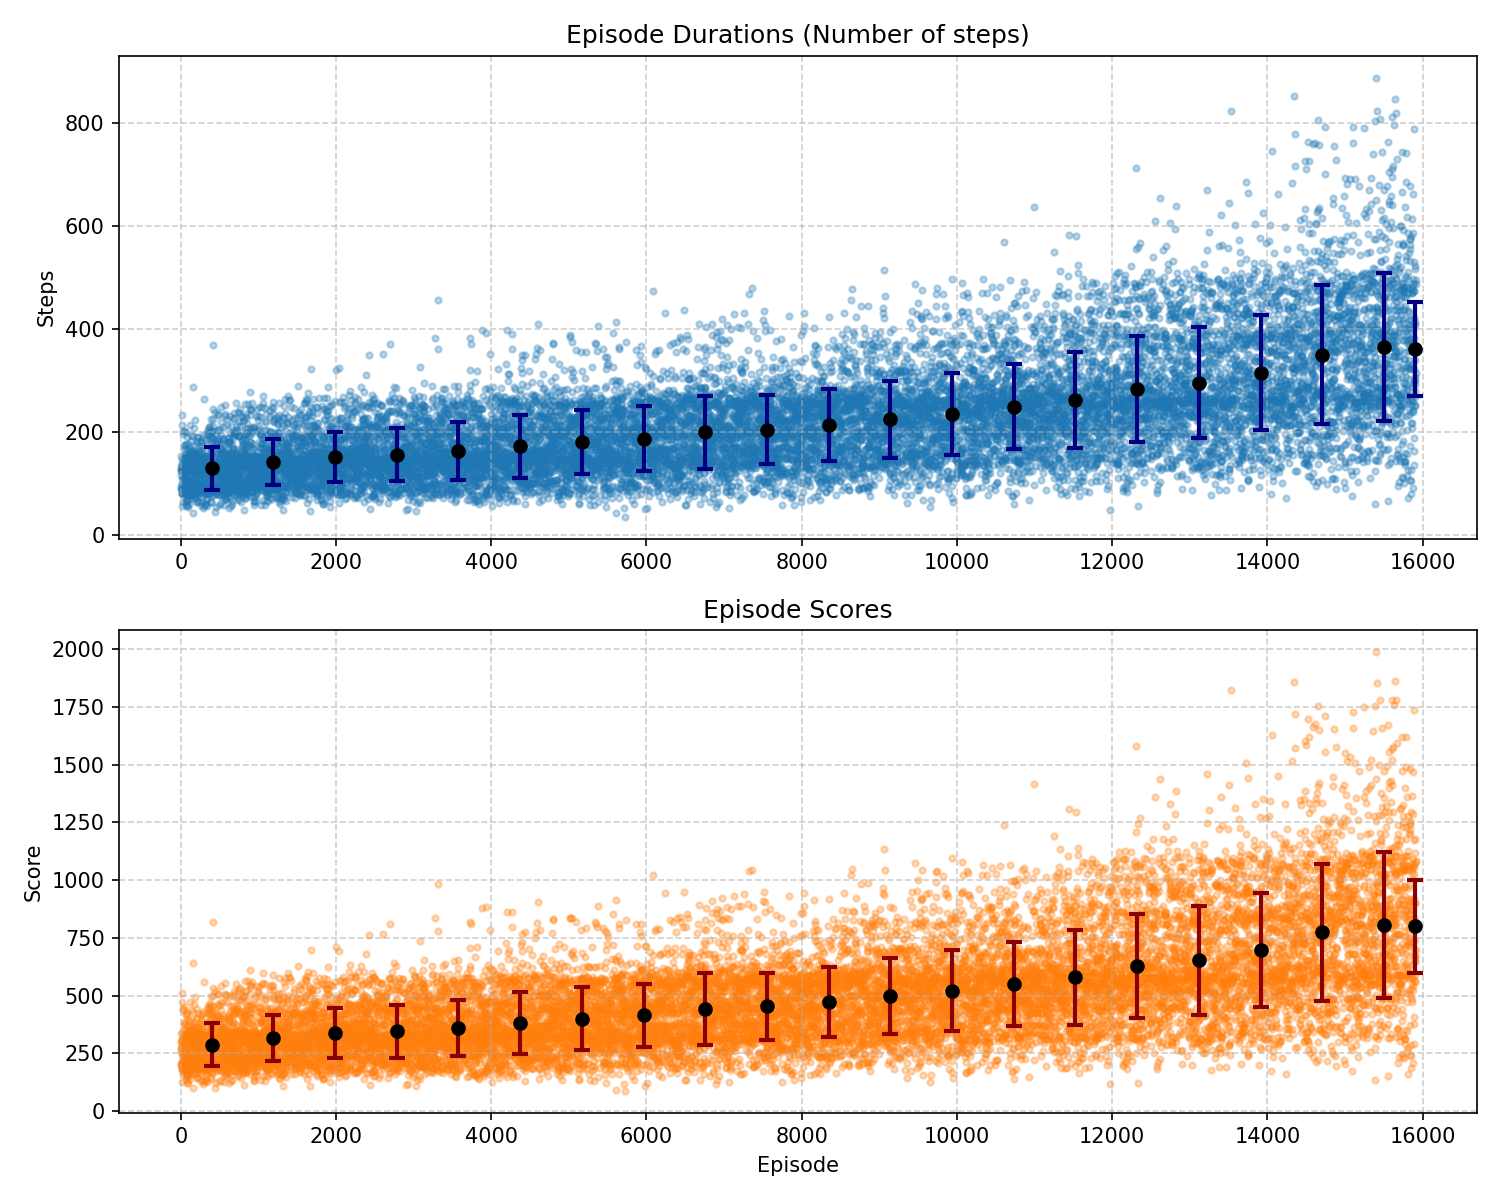
\includegraphics[width=\columnwidth]{images/dqn_learning_tracking_data.png} 
    \caption{Training metrics of the DQN learning agent. The first plot shows the average steps taken per episode, the second plot shows the average score per episode. Each plot also includes the mean and standard deviation computed over the last runs.} 
    \label{fig:dqn_training_metrics} 
\end{figure} 

\noindent The training of the TD learning agent is shown in Fig.~\ref{fig:td_training_metrics}. It trained for 50k episodes and took around 2500s to train on a CPU (i9-14900K). 

\begin{figure}[h] 
    \centering 
    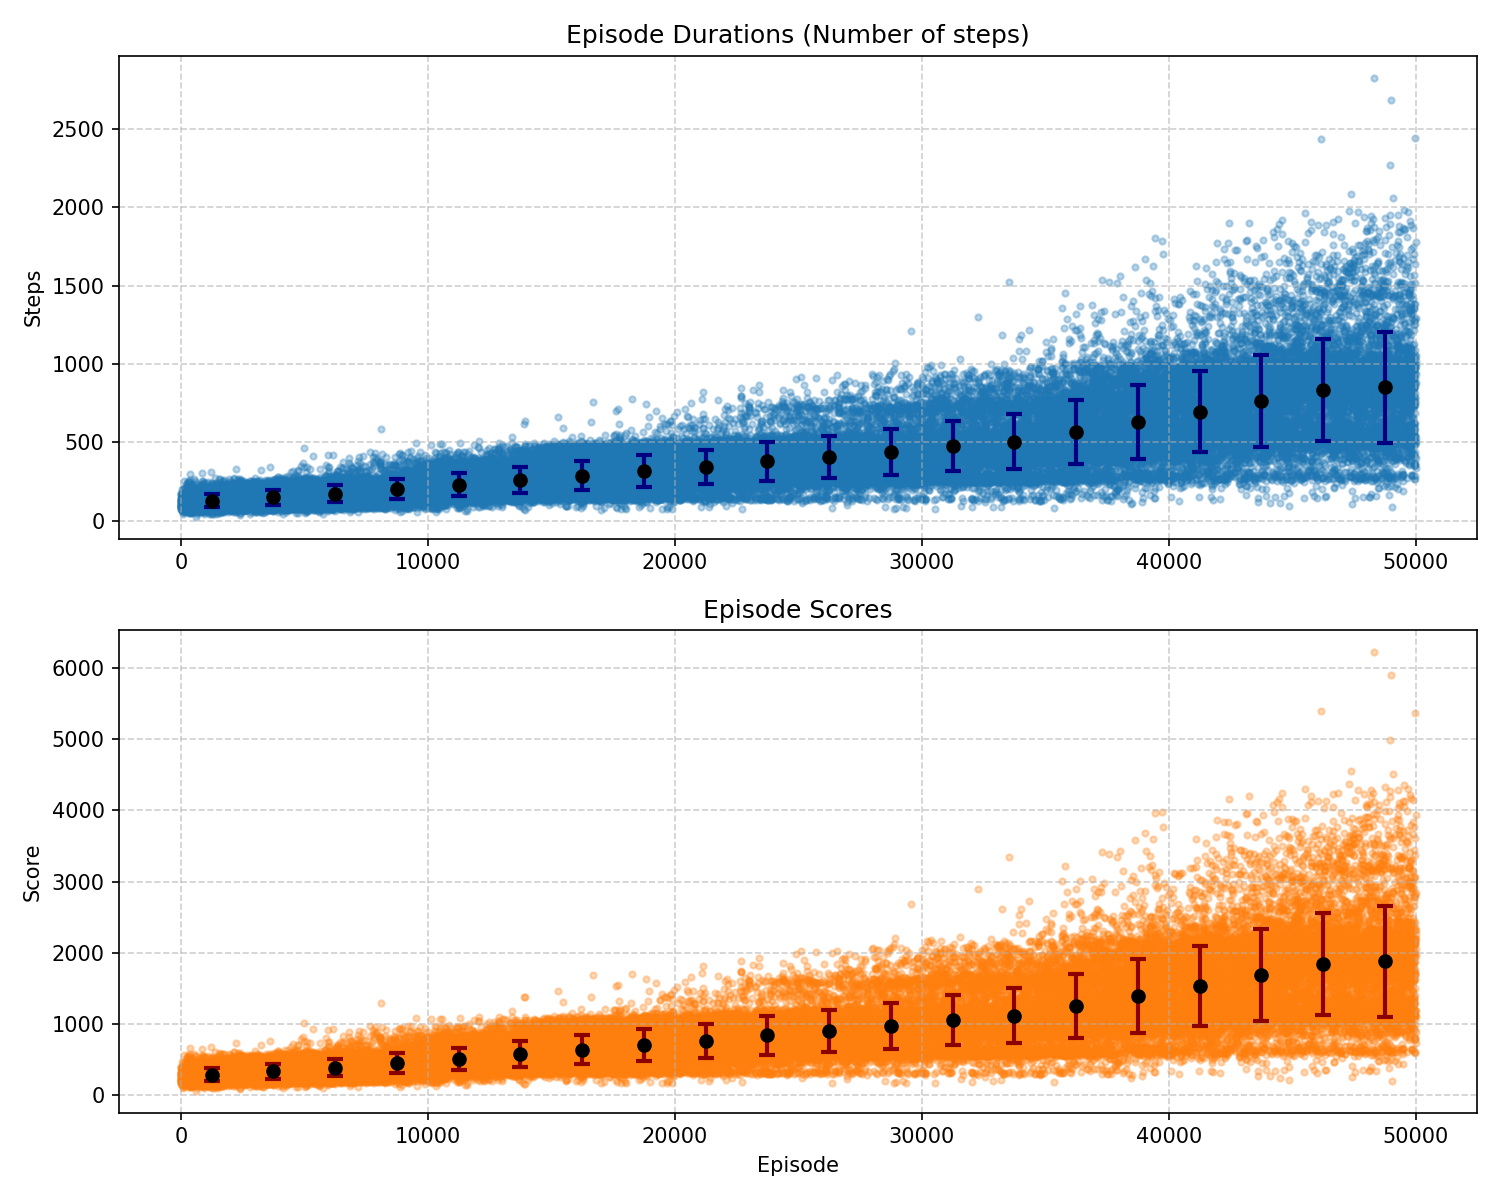
\includegraphics[width=\columnwidth]{images/td_learning_tracking_data.png} 
    \caption{Training metrics of the TD learning agent. The first plot shows the average steps taken per episode, the second plot shows the average score per episode. Each plot also includes the mean and standard deviation computed over the last runs.} 
    \label{fig:td_training_metrics} 
\end{figure}

    \noindent The TD learning agent reached a mean score of around 2000 at the end of the training while the DQN agent reached a mean score of less than 1000 even though it trained for much longer.
    This can be explained by the fact that the DQN agent is more complex due to the convolutional neural network used to approximate the Q-values, thus it requires more data and more training time to converge.

    \subsection{Evaluation metrics} \label{sb:evaluation_metrics}
    The Table \ref{tab:score_stats} present the score statistics of the three agents over 100 runs, including the mean, standard deviation, minimum and maximum scores achieved. 
    While the Table \ref{tab:time_stats} presents the time statistics of the three agents over 100 runs, including the mean, standard deviation, minimum and maximum time taken to complete a game.
    \begin{table}[H]
        \centering
        \small
        \begin{adjustbox}{max width=\columnwidth}
        \begin{tabular}{l r r r r}
        \toprule
        \textbf{Approach} & \textbf{Mean} & \textbf{Std} & \textbf{Min} & \textbf{Max} \\
        \midrule
        Expectimax       & 2721 & 1171 & 632 & 6180  \\
        Deep Q-Learning  & 1216 &  469 & 250 & 2078  \\
        N-tuple network  & 2503 &  992 & 638 & 6034 \\
        \bottomrule
        \end{tabular}
        \end{adjustbox}
        \caption{Score statistics of the three agents over 100 runs.}
        \label{tab:score_stats}
    \end{table}

    \begin{table}[H]
        \centering
        \small
        \begin{adjustbox}{max width=\columnwidth}
        \begin{tabular}{l r r r r}
        \toprule
        \textbf{Approach} & \textbf{Mean(s)} & \textbf{Std(s)} & \textbf{Min(s)} & \textbf{Max(s)} \\
        \midrule
        Expectimax       & 18.36  & 6.29 & 6.51 & 35.66  \\
        Deep Q-Learning  & 0.5144 &  0.1966 & 0.1126 & 0.8918  \\
        N-tuple network  & 0.0634 &  0.0247 & 0.0163 & 0.1522 \\
        \bottomrule
        \end{tabular}
        \end{adjustbox}
        \caption{Time statistics of the three agents over 100 runs.}
        \label{tab:time_stats}
    \end{table}

    \subsection{Statistical comparisons} \label{sb:statistical_comparisons}
    Table \ref{tab:stat_tests} presents the results of the statistical tests performed to compare the performance of the three agents based on their scores over 100 runs.
    The tests performed are the Wilcoxon signed-rank test and the Student's t-test. 
    The student's t-test is assumes a normal distribution of the scores and is thus less robust in this context but it is still interesting to keep it as a secondary test to confirm the results of the Wilcoxon test.
    A significant p-value (typically less than 0.05) indicates that there is a statistically significant difference between the two approaches being compared, 
    while a non-significant p-value suggests that any observed difference could be due to random chance.
    \begin{table}[H]
        \centering
        \small
        \begin{adjustbox}{max width=\columnwidth}
        \begin{tabular}{l l r r r r}
        \toprule
        \textbf{1st Approach} & \textbf{2nd Approach} 
            & \multicolumn{2}{c}{\textbf{Wilcoxon}} 
            & \multicolumn{2}{c}{\textbf{Student's t}} \\
        \cmidrule(lr){3-4} \cmidrule(lr){5-6}
        & & \textbf{Stat} & \textbf{p-value} & \textbf{Stat} & \textbf{p-value} \\
        \midrule
        Expectimax      & N-tuple network  & 5483 & 2.3e-01 & 1.41  & 1.6e-01 \\
        Expectimax      & Deep Q-Learning  & 8828 & 8.6e-22 & 11.86 & 1.8e-22 \\
        N-tuple network & Deep Q-Learning  & 8990 & 1.8e-22 & 11.66 & 1.9e-22 \\
        \bottomrule
        \end{tabular}
        \end{adjustbox}
        \caption{Statistical comparison of agent performances (Wilcoxon and Student's t based on scores) over 100 runs.}
        \label{tab:stat_tests}
    \end{table}

\section{Conclusion}
    As seen in the section \textit{Training metrics}\ref{sb:training_metrics}, the DQN agent requires a very long training session to reach a mean score equivalent to the TD learning agent. 
    However, with the same number of training episodes, the DQN agent performs similarly to the TD learning agent. 
    This could suggests that the primary limitation of the DQN agent is not sample efficiency but rather a more complex architecture requiring more training time to 
    converge.

    While both DQN and TD learning agents need a large amount of training data to reach good performance, 
    the Expectimax agent can reach a good performance without any training, making it a significant advantage in terms of computational cost and time.
    However, the Expectimax agent is much slower than the other two agents because of heavier computations during inference phase, causing it to be 
    a significant disadvantage in real-time applications or when computational resources are limited.

    Also, according to the sections \textit{Evaluation metrics}\ref{sb:evaluation_metrics} and \textit{Statistical comparisons}\ref{sb:statistical_comparisons}, the Expectimax and TD learning agents have similar performance in terms of score.
    but they are both significantly better than the DQN agent. A far longer training time for the DQN agent could improve it's performance but it is not guaranteed and it is not feasible for this project.

    These results demonstrate that the Expectimax agent is the best choice for this problem if instant performance is required, whereas the TD Learning agent better 
    suits scenarios where pre training is possible.  


    \begin{table}[H]
        \centering
        \small
        \begin{adjustbox}{max width=\columnwidth}
        \begin{tabular}{l r r r}
        \toprule
        \textbf{Metric} & \textbf{Expectimax} & \textbf{DQN} & \textbf{TD Learning} \\
        \midrule
        Mean score       & Highest    & Bad          & Highest    \\
        Execution time   & Highest    & Intermediate & Lowest     \\
        Training time    & None       & Highest      & Acceptable \\
        Robustness (std) & Equivalent & Equivalent   & Equivalent \\
        \bottomrule
        \end{tabular}
        \end{adjustbox}
        \caption{Approaches comparison summary.}
        \label{tab:comparison_summary}
    \end{table}

    A hybrid approach that combines TD learning and Expectimax could be an interesting direction to explore in future work, 
    where the TD learning agent could be used to learn a value function that can be used as an evaluation function for the Expectimax agent,
    which could potentially improve the performance of the Expectimax agent while keeping a reasonable computational cost.


\bibliography{aaai2026}

\end{document}
